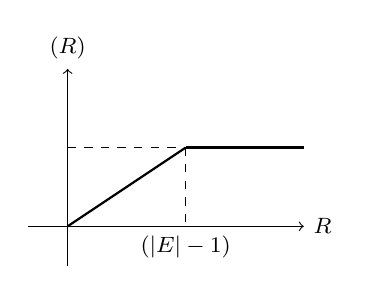
\begin{tikzpicture}
\tikzstyle{every node}=[font= \fontsize{8pt}{10pt}\selectfont]
    \draw [thin,  ->] (0,-0.5) -- (0,2)      % draw y-axis line
        node [above, black] {$\wskc(R)$};              % add label for y-axis
    
    \draw [thin,  ->] (-0.5,0) -- (3,0)      % draw x-axis line
        node [right, black] {$R$};              % add label for x-axis
    
    \draw [draw=black, thick] (0,0) -- (1.5,1);% draw the graph
    \draw [draw=black, thick] (1.5,1) -- (3,1);
    \draw [thin,  dashed] (0,1) -- (1.5,1);
    \draw [thin,  dashed] (1.5,1) -- (1.5,0);
    
    \node [left] at (0,1) {$\wskc$};                % label y-intercept
    \node [below] at (1.5,0) {$(|E|-1)\wskc$};               % label x-intercept
\end{tikzpicture}